\documentclass[11pt,a4paper]{article}

% ---------------------------------------------------------------------------
% Packages
% ---------------------------------------------------------------------------
\usepackage[T1]{fontenc}
\usepackage{lmodern}
\usepackage[margin=1in]{geometry}
\usepackage{microtype}
\usepackage{amssymb}
\usepackage{xcolor}
\usepackage{tikz}
\usetikzlibrary{shapes.multipart,arrows.meta,positioning,calc,fit,shadows,backgrounds}
\usepackage{graphicx}
\usepackage{parskip}
\usepackage{enumitem}
\usepackage{fancyhdr}
\usepackage{titlesec}
\usepackage{booktabs}
\usepackage{pdfpages}
\usepackage{hyperref}

\hypersetup{
  colorlinks=true,
  linkcolor=blue!55!black,
  citecolor=blue!55!black,
  urlcolor=blue!55!black,
  pdftitle={MatrixCanvas -- Software Design Report},
  pdfauthor={Faiyaz Tahmid, Abrar Faiyaz, Ittesaf Ithun, Tamim Naser}
}

% ---------------------------------------------------------------------------
% Colours
% ---------------------------------------------------------------------------
\definecolor{layerpres}{RGB}{219,234,254}
\definecolor{layerstate}{RGB}{254,240,199}
\definecolor{layerdomain}{RGB}{209,250,229}
\definecolor{umlfillA}{RGB}{224,231,255}
\definecolor{umlfillB}{RGB}{255,255,255}
\definecolor{boxline}{RGB}{51,65,85}

% ---------------------------------------------------------------------------
% Section styling
% ---------------------------------------------------------------------------
\titleformat{\section}{\normalfont\Large\bfseries\color{boxline}}{\thesection}{0.6em}{}
\titleformat{\subsection}{\normalfont\large\bfseries\color{boxline}}{\thesubsection}{0.6em}{}

% ---------------------------------------------------------------------------
% Header / footer
% ---------------------------------------------------------------------------
\pagestyle{fancy}
\setlength{\headheight}{14pt}
\fancyhf{}
\renewcommand{\headrulewidth}{0.4pt}
\fancyhead[L]{MatrixCanvas -- Software Design Report}
\fancyhead[R]{\thepage}
\fancyfoot[C]{\small Group Project -- Third Semester}

% ---------------------------------------------------------------------------
% UML class-box style (rectangle split: name / attributes / methods)
% ---------------------------------------------------------------------------
\tikzset{
  umlclass/.style={
    rectangle split, rectangle split parts=3,
    draw=boxline, thick, rounded corners=1.5pt,
    drop shadow={shadow xshift=1pt, shadow yshift=-1pt, opacity=0.35},
    rectangle split part fill={umlfillA,umlfillB,umlfillB},
    font=\fontsize{7.6}{9}\selectfont,
    inner sep=5pt,
    align=left
  },
  umlinterface/.style={
    rectangle split, rectangle split parts=2,
    draw=boxline, thick, rounded corners=1.5pt,
    drop shadow={shadow xshift=1pt, shadow yshift=-1pt, opacity=0.35},
    rectangle split part fill={umlfillA,umlfillB},
    font=\fontsize{7.6}{9}\selectfont,
    inner sep=5pt,
    align=left
  },
  umlrel/.style={-{Stealth[length=2.2mm]}, thick, draw=boxline},
  umldep/.style={-{Stealth[length=2.2mm]}, thick, dashed, draw=boxline!70},
  umlagg/.style={{Diamond[length=2.6mm,width=1.8mm]}-, thick, draw=boxline},
  umllabel/.style={font=\scriptsize\itshape, fill=white, inner sep=1pt}
}

\begin{document}

% =============================================================================
% TITLE PAGE
% =============================================================================
\begin{titlepage}
\centering
\vspace*{1.2cm}

{\Large \bfseries [University / Institution Name]}\\[0.3cm]
{\large [Department of Computer Science and Engineering]}\\[1.8cm]

\rule{0.85\textwidth}{0.6pt}\\[0.5cm]
{\huge \bfseries MatrixCanvas}\\[0.35cm]
{\Large An Interactive Tool for Visualising Linear Algebra Transformations}\\[0.5cm]
\rule{0.85\textwidth}{0.6pt}\\[1.2cm]

{\Large \bfseries Software Design Report}\\[0.2cm]
{\normalsize Class Diagram, Software Design Architecture Diagram \& SRS Appendix}\\[1.6cm]

{\large \bfseries Submitted by}\\[0.5cm]
\begin{tabular}{ll}
\toprule
\textbf{Name} & \textbf{Student ID} \\
\midrule
Faiyaz Tahmid  & 230042107 \\
Abrar Faiyaz   & 230042108 \\
Ittesaf Ithun  & 230042125 \\
Tamim Naser    & 230042133 \\
\bottomrule
\end{tabular}

\vfill

\begin{tabular}{ll}
\textbf{Course:}      & [Course Code -- Course Title] \\
\textbf{Instructor:}  & [Instructor Name] \\
\textbf{Submission Date:} & 26 July 2026 \\
\end{tabular}

\vspace{0.6cm}
\end{titlepage}

\tableofcontents
\newpage

% =============================================================================
\section{Introduction}
% =============================================================================

\textbf{MatrixCanvas} is a web application built to help students build geometric
intuition for $2 \times 2$ linear transformations. A user edits the four entries
of a transformation matrix and immediately sees its effect on the standard basis
vectors, the coordinate grid, and any custom vectors they add, animated smoothly
between the identity transform and the target transform. Alongside the visual,
a properties panel reports the determinant, trace, rank, eigenvalues, and
qualitative properties (invertible, orthogonal, symmetric) of the current matrix.

The application is implemented as a single-page front-end using the following
technology stack:

\begin{itemize}[nosep]
  \item \textbf{React 18} with \textbf{TypeScript} -- component-based UI, strong static typing of the domain model.
  \item \textbf{Zustand} -- a minimal, hook-based global state container.
  \item \textbf{HTML5 Canvas API} -- immediate-mode rendering of the transformed grid and vectors.
  \item \textbf{GSAP} -- tweening engine driving the identity $\rightarrow$ target animation.
  \item \textbf{React Router} -- client-side routing between the \emph{Playground} and \emph{Learn} pages.
  \item \textbf{Vite} \& \textbf{Tailwind CSS} -- build tooling and utility-first styling.

\end{itemize}

This report documents the \emph{software design} of MatrixCanvas: the object
model that underlies the application (Section~\ref{sec:class-diagram}) and the
layered architecture that organises the code base (Section~\ref{sec:architecture}).
The team's previously submitted Software Requirements Specification (SRS) is
attached as Appendix~\ref{app:srs}.

% =============================================================================
\section{Object-Oriented Design Overview}
% =============================================================================

MatrixCanvas follows an \textbf{object-oriented approach} at its core: the
mathematics of the application is encapsulated in a dedicated \texttt{Matrix2x2}
class that owns its data and exposes behaviour (determinant, trace, rank,
eigenvalues, inversion, interpolation) as methods, rather than scattering these
computations across the UI. The application's state is likewise modelled as a
strongly-typed object (\texttt{AppStore}) composed of well-defined data
interfaces (\texttt{CustomVector}, \texttt{Preset}). The presentation layer
(React components) is kept deliberately thin: components read from and write to
this object model but do not themselves hold business logic.

Because of this separation, the design is documented with the two diagrams
requested for OO projects:

\begin{enumerate}
  \item A \textbf{Class Diagram} (Section~\ref{sec:class-diagram}) of the core
        domain and state objects, their attributes, methods, and relationships.
  \item A \textbf{three-layer Software Design Architecture Diagram}
        (Section~\ref{sec:architecture}) showing how the Presentation,
        State-Management, and Domain layers are organised and how they
        communicate.
\end{enumerate}

% =============================================================================
\section{Class Diagram}
\label{sec:class-diagram}
% =============================================================================

Figure~\ref{fig:class-diagram} shows the core object model of MatrixCanvas: the
\texttt{Matrix2x2} domain class, the \texttt{AppStore} application state, and
the two plain data interfaces it depends on, \texttt{CustomVector} and
\texttt{Preset}. UI components (documented in Section~\ref{sec:architecture})
consume this model through the \texttt{useAppStore} hook and are intentionally
left out of this diagram so that the true object model stands out clearly.

\begin{figure}[htb]
\centering
\resizebox{\textwidth}{!}{%
\begin{tikzpicture}

% ---- AppStore (placed first, everything else anchors off it) ----
\node[umlclass, text width=5.4cm] (AppStore) {
  {\centering \bfseries AppStore \par}
  \nodepart{second}
  \raggedright
  -- matrixValues: Matrix2x2Values \\
  -- animProgress: number \\
  -- animTrigger: number \\
  -- customVectors: CustomVector[]
  \nodepart{third}
  + setMatrixValue(row, col, v): void \\
  + setMatrixValues(v): void \\
  + setAnimProgress(t): void \\
  + triggerAnimation(): void \\
  + addVector(x, y): void \\
  + removeVector(id): void \\
  + updateVector(id, x, y): void
};

% ---- Preset (interface) ----
\node[umlinterface, text width=3.2cm, above left=1.4cm and 2.2cm of AppStore] (Preset) {
  {\centering \scriptsize\itshape \guillemotleft interface\guillemotright\\ \bfseries Preset \par}
  \nodepart{second}
  \raggedright
  + label: string \\
  + values: Matrix2x2Values
};

% ---- CustomVector (interface) ----
\node[umlinterface, text width=3.3cm, above right=1.4cm and 2.2cm of AppStore] (CustomVector) {
  {\centering \scriptsize\itshape \guillemotleft interface\guillemotright\\ \bfseries CustomVector \par}
  \nodepart{second}
  \raggedright
  + id: string \\
  + x: number \\
  + y: number \\
  + color: string
};

% ---- Matrix2x2 ----
\node[umlclass, text width=6.2cm, below=2.6cm of AppStore] (Matrix) {
  {\centering \bfseries Matrix2x2 \par}
  \nodepart{second}
  \raggedright
  -- values: Matrix2x2Values \{readonly\}
  \nodepart{third}
  + a, b, c, d: number \{get\} \\
  + multiply(v: [number, number]): [number, number] \\
  + determinant(): number \\
  + trace(): number \\
  + rank(): number \\
  + isInvertible(): boolean \\
  + isOrthogonal(): boolean \\
  + isSymmetric(): boolean \\
  + eigenvalues(): [number, number] $\vert$ null \\
  + inverse(): Matrix2x2 $\vert$ null \\
  + lerp(target: Matrix2x2, t: number): Matrix2x2 \\
  + identity(): Matrix2x2 \{static\}
};

% ---- Relationships ----
\draw[umlagg] (AppStore.east) -- (CustomVector.south)
  node[umllabel, pos=0.12, above] {1} node[umllabel, pos=0.92, above] {0..*};

\draw[umldep] (Preset.south) -- (AppStore.west)
  node[umllabel, midway, above, sloped] {configures};

\draw[umldep] (AppStore.south) -- (Matrix.north)
  node[umllabel, midway, right] {wraps values as / uses};

\end{tikzpicture}}
\caption{Class diagram of the MatrixCanvas core object model. Solid diamond =
aggregation, dashed arrow = dependency (``uses'').}
\label{fig:class-diagram}
\end{figure}

\subsection{Explanation of the Class Diagram}

\begin{description}[leftmargin=1.4em, style=nextline]
  \item[\texttt{Matrix2x2}] is the domain class that encapsulates all linear
    algebra behaviour. It stores its four entries in a read-only
    \texttt{Matrix2x2Values} tuple and exposes accessors (\texttt{a}, \texttt{b},
    \texttt{c}, \texttt{d}) alongside computed properties -- determinant, trace,
    rank, invertibility, orthogonality, symmetry, and (real) eigenvalues -- plus
    two operational methods: \texttt{multiply} (applies the matrix to a
    2-vector) and \texttt{lerp} (linearly interpolates between two matrices,
    which drives the identity-to-target animation). \texttt{inverse} and the
    static \texttt{identity} factory return new \texttt{Matrix2x2} instances,
    keeping the class immutable.

  \item[\texttt{AppStore}] is the single source of truth for the application,
    implemented with Zustand. It holds the raw matrix values, the animation
    progress/trigger counters, and the list of user-added vectors, and exposes
    action methods that are the \emph{only} way this state may be mutated.
    Components never mutate state directly -- they call an action, and the
    store notifies all subscribers.

  \item[\texttt{CustomVector}] is a plain data interface describing one
    user-added vector (position and display colour). \texttt{AppStore}
    aggregates zero or more of these (\texttt{1} -- \texttt{0..*}); a vector's
    lifetime is entirely owned by the store.

  \item[\texttt{Preset}] is a plain data interface pairing a human-readable
    label with a canonical \texttt{Matrix2x2Values} tuple (e.g.\ ``Rotate
    45\textdegree'', ``Horizontal Shear''). Selecting a preset configures
    \texttt{AppStore} by calling \texttt{setMatrixValues}.

  \item[Dependency \texttt{AppStore} $\dashrightarrow$ \texttt{Matrix2x2}]
    reflects that the store keeps only the \emph{raw} matrix values; whenever a
    component needs derived mathematical properties or must apply the
    transform, it wraps the current \texttt{matrixValues} in a fresh
    \texttt{Matrix2x2} instance (e.g.\ \texttt{new Matrix2x2(matrixValues)} in
    \texttt{PropertiesPanel}, \texttt{VectorPanel}, and \texttt{TransformCanvas}).
    This keeps the store JSON-serialisable and the class purely computational.
\end{description}

\newpage
% =============================================================================
\section{Software Design Architecture Diagram}
\label{sec:architecture}
% =============================================================================

MatrixCanvas follows a \textbf{three-layer architecture}: a \emph{Presentation
Layer} of React components, a \emph{State-Management Layer} holding the single
Zustand store, and a \emph{Domain / Business-Logic Layer} containing the
mathematics. Figure~\ref{fig:architecture} shows the three layers and the
direction of communication between them.

\begin{figure}[htb]
\centering
\resizebox{\textwidth}{!}{%
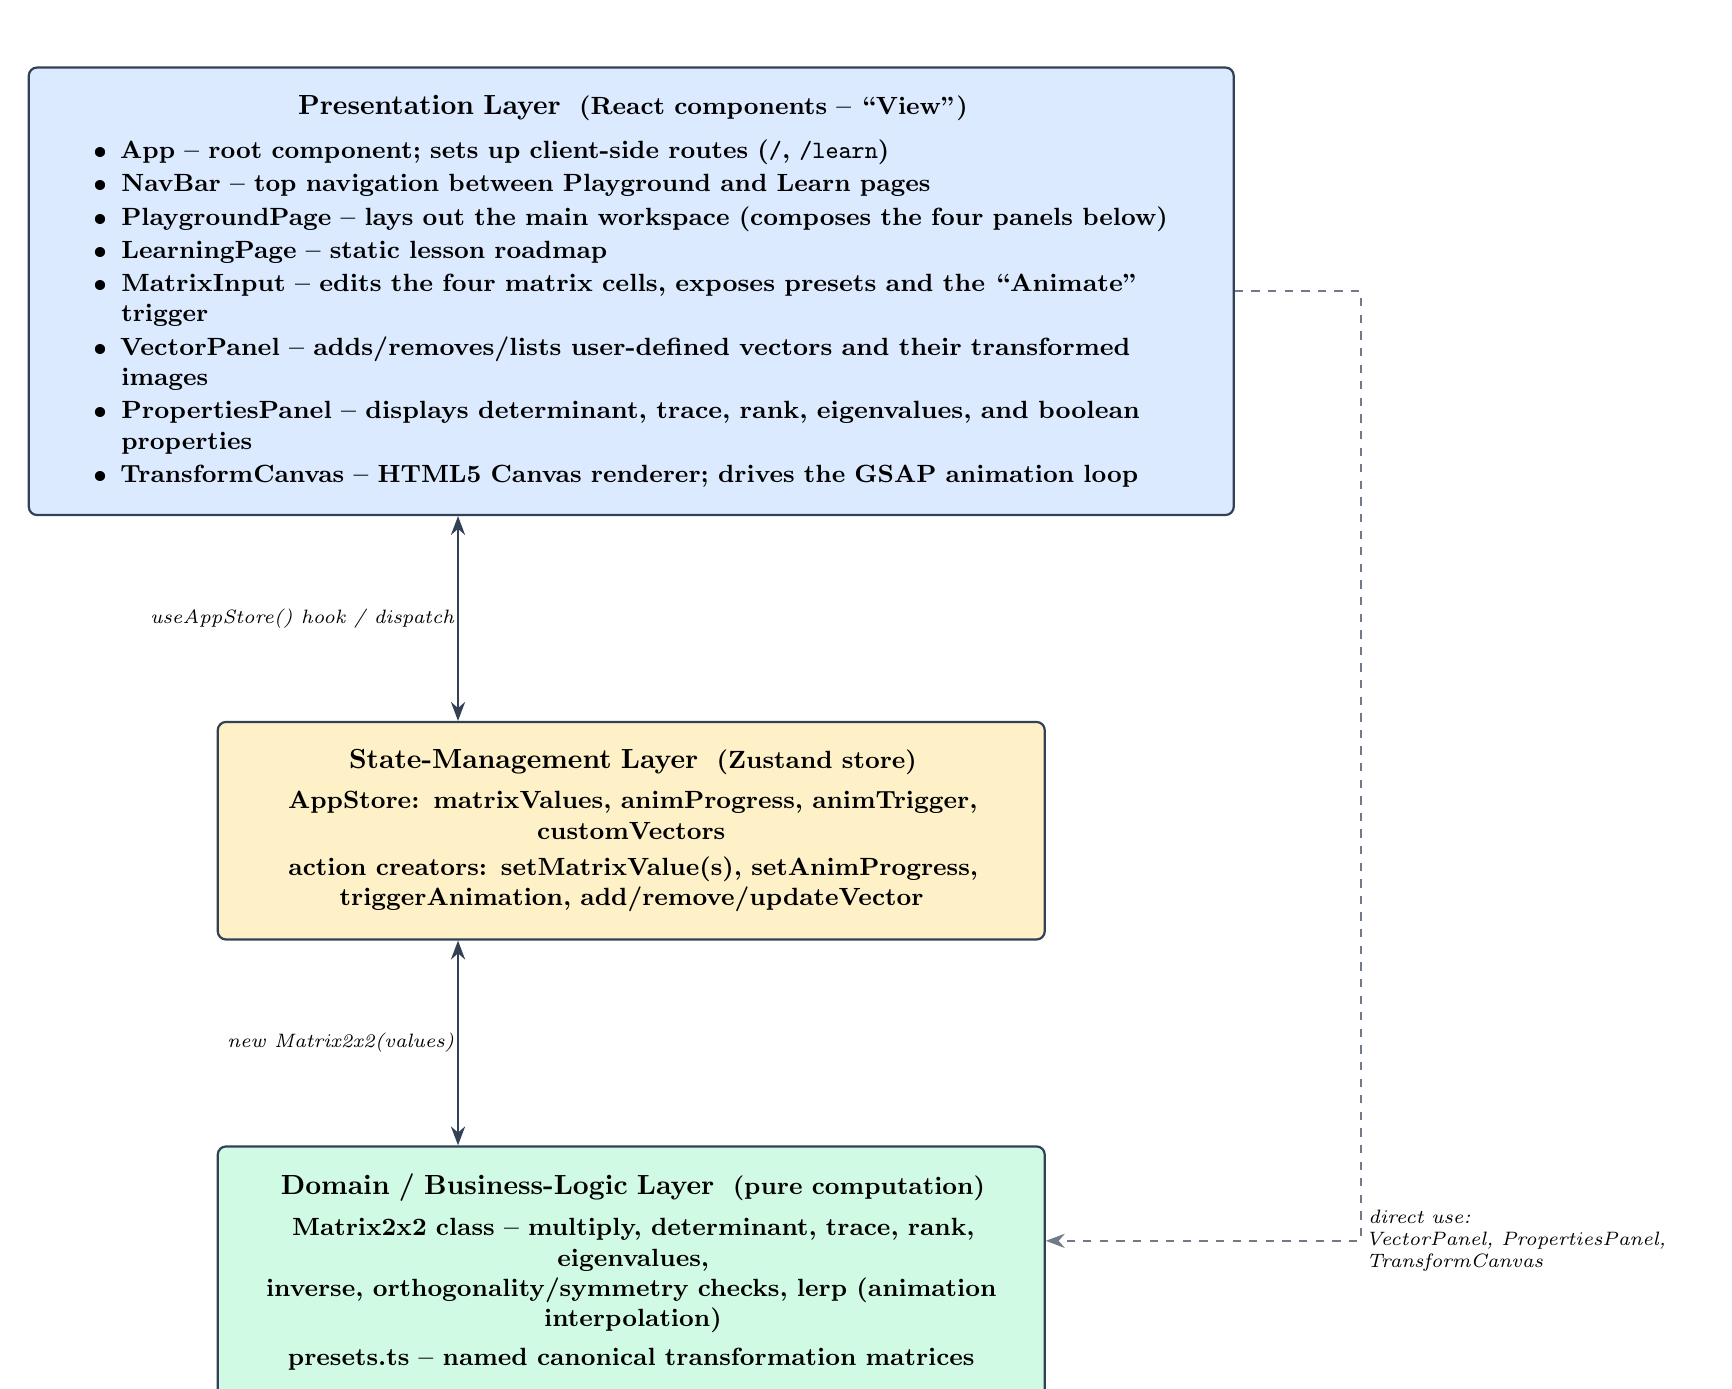
\begin{tikzpicture}[
  layerbox/.style={draw=boxline, thick, rounded corners=3pt, align=center, inner sep=10pt}
]

% ---- Presentation Layer ----
\node[layerbox, fill=layerpres, text width=14.6cm] (pres) {
  \centering \bfseries Presentation Layer \ \small(React components -- ``View'')\\[6pt]
  \begin{minipage}{14cm}
  \small
  \begin{itemize}[nosep, itemsep=1pt, leftmargin=1.4em]
    \item \textbf{App} -- root component; sets up client-side routes (\texttt{/}, \texttt{/learn})
    \item \textbf{NavBar} -- top navigation between Playground and Learn pages
    \item \textbf{PlaygroundPage} -- lays out the main workspace (composes the four panels below)
    \item \textbf{LearningPage} -- static lesson roadmap
    \item \textbf{MatrixInput} -- edits the four matrix cells, exposes presets and the ``Animate'' trigger
    \item \textbf{VectorPanel} -- adds/removes/lists user-defined vectors and their transformed images
    \item \textbf{PropertiesPanel} -- displays determinant, trace, rank, eigenvalues, and boolean properties
    \item \textbf{TransformCanvas} -- HTML5 Canvas renderer; drives the GSAP animation loop
  \end{itemize}
  \end{minipage}
};

% ---- State-Management Layer ----
\node[layerbox, fill=layerstate, text width=9.8cm, below=2.6cm of pres] (state) {
  \centering \bfseries State-Management Layer \ \small(Zustand store)\\[5pt]
  \begin{minipage}{9.4cm}
  \small
  \centering
  \textbf{AppStore}: matrixValues, animProgress, animTrigger, customVectors\\[2pt]
  action creators: setMatrixValue(s), setAnimProgress, triggerAnimation, add/remove/updateVector
  \end{minipage}
};

% ---- Domain Layer ----
\node[layerbox, fill=layerdomain, text width=9.8cm, below=2.6cm of state] (domain) {
  \centering \bfseries Domain / Business-Logic Layer \ \small(pure computation)\\[5pt]
  \begin{minipage}{9.4cm}
  \small
  \centering
  \textbf{Matrix2x2} class -- multiply, determinant, trace, rank, eigenvalues,\\
  inverse, orthogonality/symmetry checks, lerp (animation interpolation)\\[3pt]
  \textbf{presets.ts} -- named canonical transformation matrices
  \end{minipage}
};

% ---- Arrows between layers ----
\draw[umlrel, {Stealth[length=2.4mm]}-{Stealth[length=2.4mm]}]
  ($(pres.south)+(-2.2,0)$) -- ($(state.north)+(-2.2,0)$)
  node[umllabel, midway, left] {useAppStore() hook / dispatch};

\draw[umlrel, {Stealth[length=2.4mm]}-{Stealth[length=2.4mm]}]
  ($(state.south)+(-2.2,0)$) -- ($(domain.north)+(-2.2,0)$)
  node[umllabel, midway, left] {new Matrix2x2(values)};

% ---- Direct shortcut: some components use Matrix2x2 straight from props/state ----
\draw[umldep, -{Stealth[length=2.4mm]}]
  (pres.east) -- ++(1.6,0) |- ($(domain.east)+(0,0.4)$)
  node[umllabel, pos=0.5, align=left, text width=4.2cm, anchor=west, xshift=2pt]
    {direct use:\\ VectorPanel, PropertiesPanel,\\ TransformCanvas};

\end{tikzpicture}}
\caption{Three-layer software design architecture of MatrixCanvas. Solid
double-headed arrows show the normal read/write flow through the state layer;
the dashed arrow shows components instantiating \texttt{Matrix2x2} directly
for derived computations.}
\label{fig:architecture}
\end{figure}

\subsection{Explanation of the Architecture Diagram}

\begin{description}[leftmargin=1.4em, style=nextline]
  \item[Presentation Layer] contains every React component. Its only
    responsibilities are rendering and capturing user input (typing matrix
    values, adding a vector, clicking ``Animate''). It never computes a
    determinant or an eigenvalue itself.

  \item[State-Management Layer] is the single \texttt{AppStore} created with
    Zustand. Every component that needs live data calls the
    \texttt{useAppStore} hook (a selector subscription), and every user action
    is expressed as a call to one of the store's action methods -- this keeps
    all state transitions in one auditable place. \texttt{TransformCanvas}
    additionally uses \texttt{useAppStore.subscribe} to mark its canvas
    ``dirty'' and redraw on the next animation frame, instead of re-rendering
    the whole React tree on every tick.

  \item[Domain / Business-Logic Layer] contains \texttt{Matrix2x2} and
    \texttt{presets.ts}. This layer has no knowledge of React or Zustand: it is
    plain, unit-testable TypeScript that could be reused in a completely
    different UI.

  \item[Layer communication] is intentionally not a strict pass-through: while
    \texttt{MatrixInput} only ever touches the State layer (it edits raw
    numbers), \texttt{VectorPanel}, \texttt{PropertiesPanel} and
    \texttt{TransformCanvas} read the raw \texttt{matrixValues} out of the
    store and then construct a \texttt{Matrix2x2} locally to obtain derived
    values or apply the transform. This shortcut (dashed arrow) avoids storing
    derived, recomputable data in global state.
\end{description}

% =============================================================================
\section{Conclusion}
% =============================================================================

The class diagram and the three-layer architecture diagram together describe
how MatrixCanvas is designed: a small, immutable \texttt{Matrix2x2} domain
class carries all linear-algebra behaviour; a single Zustand \texttt{AppStore}
mediates all state changes; and a purely presentational React component tree
renders the result and forwards user intent back to the store. This separation
keeps the mathematics testable in isolation from the UI, and keeps the UI free
of business logic. The team's full functional and non-functional requirements
are documented in the attached SRS (Appendix~\ref{app:srs}).

\newpage
\appendix
% =============================================================================
\section{Software Requirements Specification}
\label{app:srs}
% =============================================================================

The Software Requirements Specification (SRS) previously submitted for this
project is attached below.

\bigskip
\noindent\emph{Instructions for the team: export your SRS document to a PDF
named \texttt{srs.pdf}, place it in this same folder, and uncomment the line
below (requires the \texttt{pdfpages} package, already loaded at the top of
this file).}

% \includepdf[pages=-, pagecommand={\thispagestyle{fancy}}]{srs.pdf}

\end{document}
